\documentclass{standalone}
\usepackage{diplomski}

\begin{document}

\chapter{Fibre-optic technology} \label{ch:fibres}
\pagenumbering{arabic}
\setcounter{page}\thestranica

% --------------------------------------

An optical fibre enables propagation of light by means of total reflection occurring within its core. Fibres consist of a number of cylindrical layers, the innermost being the core, surrounded by cladding. The two layers are further enclosed in a jacket, following a number of shields and isolation materials, depending on the required cable rigidity and specified applications \cite{fer:oks}. A number of standard types of fibre-optic cables are used in communication systems. These differ by their geometry and the type of optical signal they are able to guide. \\

In order for the light to be guided within the fibre, total reflection against core's boundaries must be ensured to keep the light confined. A geometric-optical interpretation of this mechanism is presented in Figure \ref{fig:critical_angle}.
\begin{figure}[h]
	\centering
	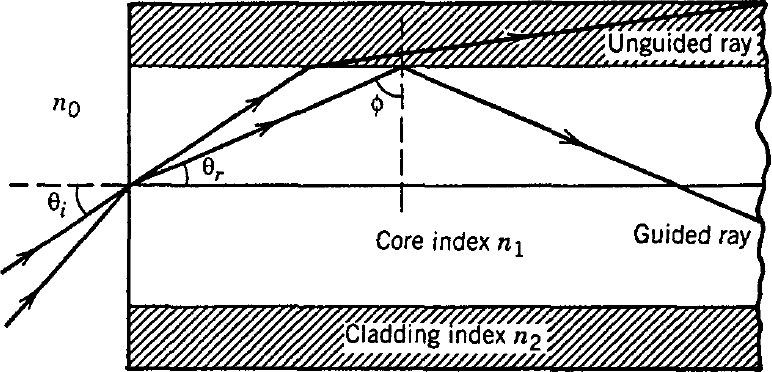
\includegraphics[width=0.6\textwidth]{critical_angle.png}
	\caption{Guiding of light in an optical fibre \cite{agrawal}}
	\label{fig:critical_angle}
\end{figure}
A critical angle $\phi_C$ is defined as the maximum incident angle of light to the core boundary, so that the light is still reflected against it. The angle is defined as
\begin{equation}
\sin \phi_C = n_2/n_1 \textrm{,}
\end{equation}
where $n_1$ is the refractive index of the core, and $n_2$ the refractive index of the cladding. The term is a result of the limitations imposed by Snell's law. Another characteristic of fibres is the \textit{numerical aperture} that represents the light gathering capacity of a fibre \cite{agrawal}. It can be expressed as 
\begin{equation}
\textrm{NA} = n_1 \, \sqrt{2 \varDelta}
\end{equation}
\begin{equation}
\varDelta = \frac{n_1 - n_2}{n_1} \textrm{.}
\end{equation}
These parameters also define the maximum bit-rate-length multiple. As the light propagates, multiple geometrical paths can occur, leading to an arrival-time delay. This phenomenon is referred to as \textit{multipath dispersion}, and is a limiting factor of the bit-rate-length multiple. To reduce the effects of multipath dispersion, graded-index fibres can be used, as opposed to step-index fibres. A comparison of their reflection index profiles is presented in Figure \ref{fig:index_profiles}.
\begin{figure}[h]
	\centering
	\begin{subfigure}[b]{0.6\textwidth}
		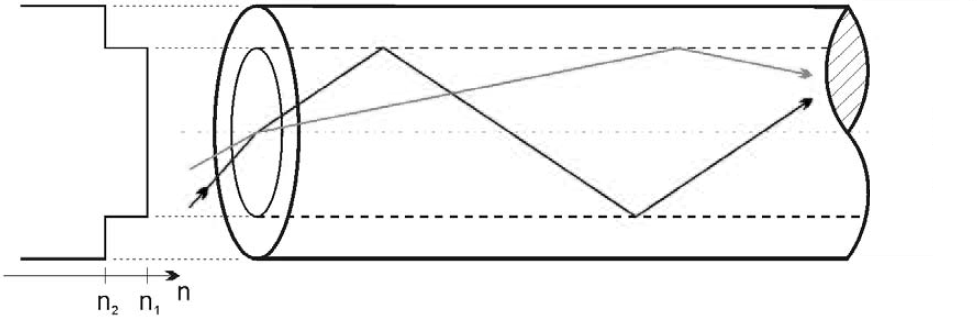
\includegraphics[width=\textwidth]{index_profiles_step.png}
		\caption{Step index profile}
		\vspace*{1em}
	\end{subfigure}
	\begin{subfigure}[b]{0.6\textwidth}
		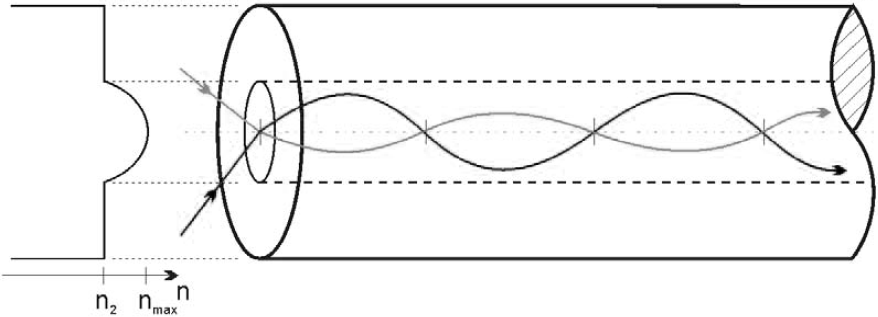
\includegraphics[width=\textwidth]{index_profiles_graded.png}
		\caption{Graded index profile}
	\end{subfigure}
	\caption{Fibre index profiles  \cite{fer:oks}}
	\label{fig:index_profiles}
\end{figure}
The gradual decrease in core's refractive index leads to better light confinement towards the centre axis of the fibre core. Thus, multipath dispersion effects will be smaller.\\

Light propagating in the optical fibre can also be observed as a travelling wave. Its propagation is governed by the wave equation
\begin{equation} \label{eq:wave}
\nabla^2 \mathbf{E} + n^2(r,\omega) \, k_0^2 \, \mathbf{E} = 0 \textrm{.}
\end{equation}
The refractive index is taken as wavelength-dependant, and the free-space wave number $k_0$ is
\begin{equation}
k_0 = \frac{\omega}{c} = \frac{2 \pi}{\lambda} \textrm{.}
\end{equation}
By solving the equation \ref{eq:wave}, one can obtain multiple solutions, each corresponding to one \textit{fibre mode} that is uniquely determined by its propagation constant $\beta_{nm}$. Each mode has its own \textit{mode index}, or \textit{effective index}, determined as
\begin{equation}
\overline{n} = \beta/k_0 \textrm{,}
\end{equation}
and whose value lies within $n_1 > \overline{n} > n_2$. At $\overline{n} = n_2$, the mode in question is said to be in \textit{cut-off}, and is no longer guided. The parameter $V$, called \textit{normalized frequency}, is used to determine the cut-off condition.
\begin{equation}
V = k_0 \, a \, \sqrt{n_1^2 - n_2^2} \approx \frac{2 \pi}{\lambda} a n_1 \sqrt{2 \varDelta}
\end{equation}
Here, $a$ is the core radius. \\

For fibres with $V < 2.405$ only the fundamental mode is guided. Such fibres are, therefore, called \textit{single-mode} fibres (abbr. SMF). Taking typical values of $n_1 = 1.45$, $\varDelta = 5 \times 10^{-3}$, $\lambda = \SI{1.55}{\micro \meter}$, we find that the core radius should be no larger than $a < \SI{4.09}{\micro \meter}$. A typical SMF has a core diameter of 8 \textmu m. Fibres with a value of $V$ larger than 2.405 are called \textit{multi-mode} fibres (abbr. MMF), as they guide a larger number of modes. Typically, MMFs have a core diameter of 50 \textmu m, 62.5 \textmu m or 125 \textmu m.


\section{Fibre losses and linear effects}

In modern communication applications, optical fibres pose the best data transfer medium. The qualities of an optical fibre supersede those of electrical conductors. Firstly, optical fibres employ a much higher frequency range, enabling broad-spectrum data transfer. The medium is, thus, utilized to a much greater extent than, for example, a coaxial cable operating in ultra-high frequency range under 1 GHz. Also, optical fibres have proven to be much more durable in terms of both mechanical endurance and immunity to electromagnetic interference. In communication and sensing applications, optical fibres represent a reliable, resilient medium. \\

Under normal conditions, the attenuation of optical power in a fibre is governed by Beer's law. Optical power at any point can be expressed as
\begin{equation}
P(z_0) = P_\textrm{in} \exp\left(-\alpha z_0\right) \textrm{,}
\end{equation}
where $\alpha$ is the attenuation coefficient in units of Np/km. For convenience, $\alpha$ is usually expressed in units of dB/km. The two units are related as
\begin{equation}
\alpha \,\textrm{[dB/km]} = 10\log(e) \cdot \alpha \,\textrm{[Np/km]} \approx 4.343 \cdot \alpha \,\textrm{[Np/km]} \textrm{.}
\end{equation}
Losses in a fibre depend on the optical wavelength. In communication systems, three \emph{optical communication windows} were defined by wavelengths at which silica fibre exhibits minimum losses. The first is around 850 nm (nowadays used only in local communication networks), the second around 1310 nm and the third around 1550 nm. These windows are the result of wavelength-dependent material absorption, i.e. the absorption by fused silica, that features minimum contribution at wavelengths around these windows, but exhibits high losses at some other characteristic wavelengths. The source of other losses is, by a large extent, Rayleigh scattering, which is a fundamental loss mechanism. It arises from microscopic density fluctuations of silica that lead to refractive index fluctuations on a scale smaller than the optical wavelength. The contribution of Rayleigh scattering to the overall fibre loss can be expressed as
\begin{equation} \label{eq:rayleigh_loss}
\alpha_\textrm{R} = C / \lambda^4 \textrm{.}
\end{equation}
Here, $C$ is a fibre-dependent constant, ranging around $\SI{0.7}{(\decibel / \kilo \meter) \, \micro \meter ^4} < C < \SI{0.9}{(\decibel / \kilo \meter) \, \micro \meter ^4}$, producing a Rayleigh-limited attenuation coefficient around $\SI{0.12}{\decibel / \kilo \meter} < \alpha_R < \SI{0.16}{\decibel / \kilo \meter}$ at the wavelength of 1.55 \textmu m. Rayleigh scattering is largely dependent on wavelength. \\

The propagation constant $\beta$ is frequency-dependent. Therefore, its frequency-dependent expression is also known as \textit{the dispersion relation} \cite{chalmers:foc}. It can be expanded into Taylor's series
\begin{equation}
\beta(\omega) = \beta_0 + \beta_1 \frac{d \beta}{d \omega} + \frac{1}{2} \beta_2 \frac{d^2 \beta}{d \omega^2} + \frac{1}{6} \beta_3 \frac{d^3 \beta}{d \omega^3} + \dots \, \textrm{.}
\end{equation}
A number of important coefficients are defined here, the first being $\beta_0$, which defines the phase velocity of a monochromatic wave
\begin{equation}
v_p = \frac{\omega_0}{\beta_0} \textrm{.}
\end{equation}
The next, $\beta_1$ is the group velocity dispersion parameter. It defines pulse broadening during propagation, which leads to a linear effect of dispersion. The total dispersion can be expressed as
\begin{equation}
\varDelta T = L \beta_2 \varDelta \omega \textrm{,}
\end{equation}
where $\varDelta \omega$ is the frequency spread of the optical signal. Parameter $\beta_2$ describes the material dispersion and waveguide dispersion, while higher-order dispersions are also governed by term $\beta_3$. It is clear that the dispersion poses a major limiting factor in long-haul or high-bit-rate communications.

\section{Non-linear optical effects}

\subsection{Phase-modulating effects}

Due to its imperfectly cylindrical shape, every fibre exhibits \textit{birefringence}. Two orthogonally polarized modes no longer propagate along the fibre independently, but instead exchange their powers, as presented in Figure \ref{fig:birefringence}.
\begin{figure}[h]
	\centering
	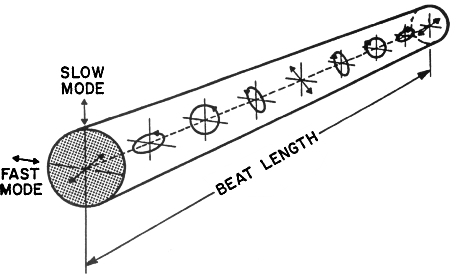
\includegraphics[width=0.6\textwidth]{birefringence.png}
	\caption{Polarization state exchange in a birefringent fibre \cite{agrawal}}
	\label{fig:birefringence}
\end{figure}
This is due to different refractive indices on two axes, $\overline{n_x}$ and $\overline{n_y}$. They are commonly related by a quantity called \textit{birefringence}
\begin{equation}
B_m = \left| \overline{n_x} - \overline{n_y} \right| \textrm{.}
\end{equation}
The \textit{beat length} is obtained as
\begin{equation}
L_B = \lambda / B_m \textrm{.}
\end{equation} \\

Fundamental non-linear effects are self-phase modulation (abbr. SPM) and cross-phase modulation (abbr. XPM). The former is the result of a power-dependant propagation constant
\begin{equation}
\beta(P) = \beta + k_0 \frac{\overline{n_2} P}{A_\textrm{eff}} = \beta + \gamma P \textrm{,}
\end{equation}
where $\overline{n_2}$ is the non-linear index coefficient, and $\gamma$ a \textit{non-linear parameter}. The phase shift for SPM can be obtained as
\begin{equation}
\phi_\textrm{SPM} = \gamma P_\textrm{in} L_\textrm{eff} \textrm{.}
\end{equation}
The $L_\textrm{eff}$ is the effective interaction length, that compensates for fibre attenuation. It is found as
\begin{equation} \label{eq:leff}
L_\textrm{eff} = \frac{1 - \exp\left(-\alpha \, L\right)}{\alpha} \approx \frac{1}{\alpha} \textrm{.}
\end{equation}
Similarly to the propagation constant, the refractive index is also power-dependent.
\begin{equation}
n(P) = \overline{n_0} + \overline{n_2} \frac{P}{A_\textrm{eff}} \textrm{.}
\end{equation}
Here, $\overline{n_0}$ is the \textit{linear refractive index}. Fibres with a large $\overline{n_2}$ are called highly non-linear fibres \cite{Hiroishi2003}. If a number of signals are transmitted through a fibre in a wave-division multiplex (abbr. WDM), optical powers of all multiplexed signals will contribute to an increase in $\beta$ and $n$. Therefore, the phase shift for the worst-case scenario in channel $i$ is given as
\begin{equation}
\phi_{i,\textrm{NL}} = \gamma L_\textrm{eff} \left( P_i + 2 \sum_{j\ne i} P_j \right) \textrm{.}
\end{equation}
A special case of XPM, when very short optical pulses are being sent, is non-dispersive XPM. Due to birefringence, two orthogonal components will interact, causing phase shifts in each component at a single wavelength
\begin{subequations}
	\begin{equation}
	\phi_x = \gamma \left(P_x + B P_y\right) L_\textrm{eff}
	\end{equation}
	\begin{equation}
	\phi_y = \gamma \left( P_y + B P_x \right) L_\textrm{eff} \textrm{.}
	\end{equation} 
\end{subequations}
The total phase shift from SPM and non-dispersive XPM is given as
\begin{equation}
\phi_\textrm{XPM} = \gamma L_\textrm{eff} \left(1 - B\right) \left(P_x - P_y\right) \textrm{.}
\end{equation} \\

In communication systems, the maximum tolerable phase shift is taken as $\phi_\textrm{NL} < 0.1$. Therefore, communication systems use power levels that are not to exceed
\begin{equation}
P_\textrm{in} < 0.1 \frac{\alpha}{\gamma} \frac{1}{N_A} \textrm{,}
\end{equation}
where $N_A$ is the number of amplifiers used. Therefore, SPM alone is a major limiting factor in long-haul optical systems.


\subsection{Brillouin scattering}

In distributed temperature sensing systems (abbr. DTS), two non-linear scattering effects can be effectively used \cite{epflBookInelastic}. The first is Brillouin effect. It is a result of the electrostriction phenomenon, i.e. the compression of the material in the presence of an electromagnetic field \cite{agrawalNonlinear}. The optical pulse functions as a pump, exciting molecules in the fibre from the ground state into a higher, virtual state. The decay of these states will produce a Stokes component -- with the wavelength being longer than that of the incident optical wave -- or an anti-Stokes component, with the wavelength being shorter than that of the incident optical wave. An illustration of this shift is given in Figure \ref{fig:freq_shift}.
\begin{figure}[h]
	\centering
	\begin{subfigure}[b]{0.35\textwidth}
		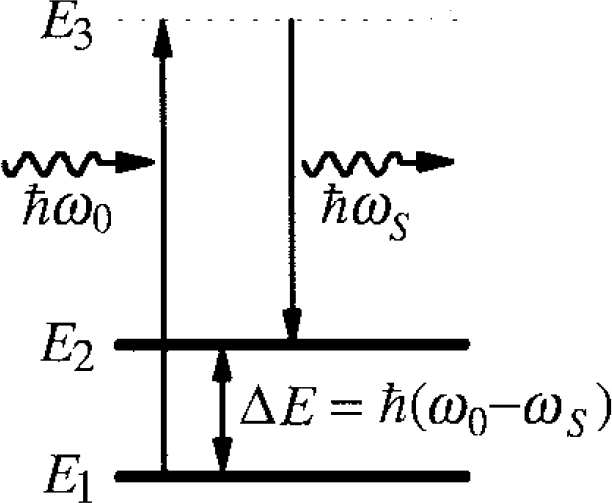
\includegraphics[width=\textwidth]{freq_shift_stokes.png}
		\caption{Stokes shift}
	\end{subfigure}
	\begin{subfigure}[b]{0.35\textwidth}
		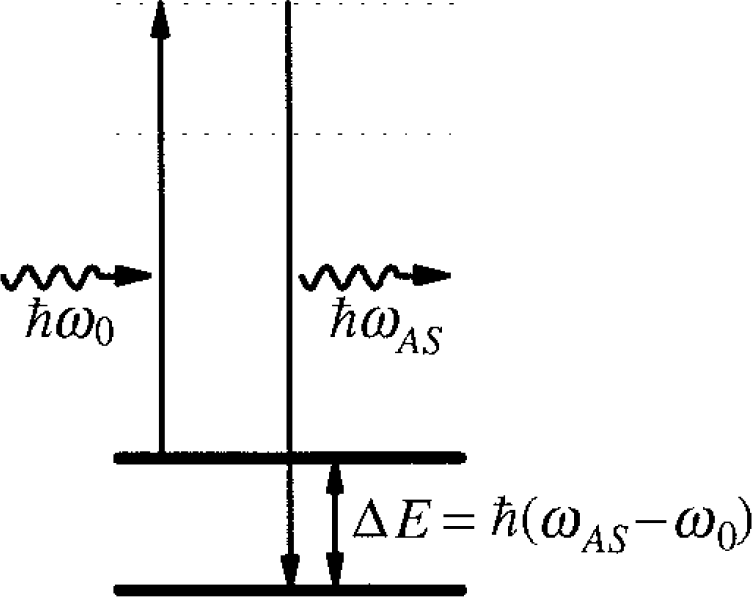
\includegraphics[width=\textwidth]{freq_shift_antistokes.png}
		\caption{Anti-Stokes shift}
	\end{subfigure}
	\caption{Frequency shifts in energy diagram \cite{Farahani1999}}
	\label{fig:freq_shift}
\end{figure}
The shift will create phonons, i.e. an acoustic wave at frequency
\begin{equation}
\Omega = \left|k_A\right| \, v_A = 2 v_A \, \left|k_p\right| \, \sin\left(\theta / 2 \right) \textrm{,}
\end{equation}
where wave vectors $k_A = k_P - k_S$ correspond to acoustic, pump and Stokes waves, respectively. Term $v_A$ is the acoustic velocity, and $\theta$ the angle between the pump and scattered waves. Note that, due to the term $\sin\left(\theta / 2\right)$, the produced wave will not propagate in forward direction, but it will be maximum in backward direction. The Brillouin shift is given as
\begin{equation}
\nu_B = \pm \frac{\Omega_B}{2 \pi} = \pm \frac{2 n_g v_A}{\lambda_P} \textrm{.}
\end{equation}
For silica fibre, and a typical pump wavelength of 1.55 \textmu m, the frequency shift is about 
\begin{equation}
\nu_B = \SI{11.1}{\giga \hertz} \textrm{.}
\end{equation}
This frequency shift can easily be monitored by radio-frequency electronics. The value of the frequency shift is temperature- and strain-dependent. Typically, the Brillouin frequency shift advances at rates about $C_{\nu\theta} = \SI{1.10}{\mega \hertz \, \kelvin^{-1}}$ and $C_{\nu\epsilon} = \SI{48}{\kilo \hertz \, \epsilon^{-1}}$. The width of Stokes and anti-Stokes lines is typically 30 -- 40 MHz. Monitoring the central frequencies, one can obtain the information about temperature and strain along the fibre. \\

This measurement method will be efficient in the spontaneous Brillouin scattering regime. In it, the scattered wave is generated spontaneously, as fibre molecules are already thermally excited. Provided the incident optical power is large enough, the produced scattered wave will beat with the pump wave, increasing the amplitude of the scattered wave. Such a phenomenon is then referred to as the stimulated Brillouin scattering (abbr. SBS). In order for simulated scattering to occur, the pump pulse power must be over the threshold level. This level is dependent on Brillouin gain $g_B$, and the effective cross-section area of the fibre in question 
\begin{equation}
A_\textrm{eff} = \pi \, w^2 \textrm{,}
\end{equation}
with $w$ being the spot size. The threshold is given as
\begin{equation}
P_\textrm{th} \approx 21 \cdot \frac{A_\textrm{eff}}{g_B \, L_\textrm{eff}} \textrm{,}
\end{equation}
where $L_\textrm{eff}$ is the same as in \ref{eq:leff}. Some methods for measuring temperature or strain by using stimulated Brillouin scattering exist, employing an excitation laser at each end of the measurement fibre \cite{Rogers1999}. This, however, requires excellent source coherence, and it is also impossible to measure temperature and strain simultaneously. Such a measurement fibre could hardly be used for communication purposes in parallel. The stimulated Brillouin scattering method, also dubbed \textit{loss Brillouin OTDR}, can nevertheless prove advantageous in long-haul measurements.

\subsection{Raman scattering}
The other effect used in distributed temperature sensing systems is the Raman effect. It is a result of molecular vibrations and rotations modulating the incident optical light. The same phenomenon of photon absorption and re-emission occurs as in Figure \ref{fig:freq_shift}, only this time no acoustic phonons are involved. Therefore, Raman scattering is an isotropic process, and scattering occurs in all directions. In the Raman effect, vibrational energy levels of fibre structure dictate the value of Raman shift
\begin{equation}
\Omega_R = \omega_P - \omega_S \textrm{.}
\end{equation}
Similarly as in Brillouin effect, Stokes and anti-Stokes shifts are defined. Photons produced by the Stokes shift will have the wavelength $\lambda_S$ -- longer than that of the incident pump -- and those produced by the anti-Stokes shift will have the wavelength $\lambda_{AS}$, shorter than that of the optical pump. The total optical power produced by the Stokes shift can be obtained from 
\begin{equation} \label{eq:raman_beer}
dP_S = P_0 \, \rho_S \, \Gamma_S \, dz \textrm{,}
\end{equation}
where $P_0$ is the incident optical pulse power, and $\Gamma_S$ the coefficient of scattering capture, dependent on fibre's geometry and Stokes wavelength. The Bose-Einstein distribution $\rho_S$ is temperature dependent as
\begin{equation} \label{eq:be-s}
\rho_S \propto \frac{1}{1- \exp\left( - \frac{\varDelta E}{k T} \right)} \textrm{.}
\end{equation}
The energy shift $\varDelta E$ can be expressed as
\begin{equation}
\varDelta E = \hbar \left( \omega_P - \omega_S \right) \textrm{.}
\end{equation}
A similar differential power expression can be expressed for the anti-Stokes shift, with a different term for the Bose-Einstein distribution
\begin{equation} \label{eq:be-as}
\rho_{AS} \propto \frac{\exp\left( - \frac{\varDelta E}{k T} \right)}{1 - \exp\left( - \frac{\varDelta E}{k T} \right)} \textrm{.}
\end{equation}
Here, $\varDelta E$ is defined as
\begin{equation}
\varDelta E = \hbar \left( \omega_P - \omega_{AS} \right) \textrm{.}
\end{equation}
The different distribution terms arise from the fact that anti-Stokes radiation produces photons of larger energy than the incident pump photon. The energy difference must be provided by the excited molecule itself, and therefore the term must account for the number of molecules available in the proper vibrational state. It is now clear that both shifted components have a temperature dependence, but also that the dependence is much larger for the anti-Stokes component. \\

Typically, a Raman shift is about 13 THz, which is far larger than Brillouin shift. Thus, for the incident wavelength of
\begin{equation}
\lambda_0 = \SI{1550}{\nano \meter}
\end{equation}
Stokes and anti-Stokes central wavelengths are around
\begin{subequations}
	\begin{equation}
	\lambda_S = \SI{1650}{\nano \meter}
	\end{equation}
	\begin{equation}
	\lambda_{AS} = \SI{1450}{\nano \meter} \textrm{.}
	\end{equation}
\end{subequations}
Such frequency shifts can not be observed in the electrical domain, as was the case for Brillouin shifts. Signals at new wavelengths will have to be monitored optically. In this case, temperature information is not coded in the spectrum of scattered signals, but rather in the amplitude. Therefore, Raman-shifted components can be optically filtered and easily detected. \\

In equations \ref{eq:be-s} and \ref{eq:be-as}, one can observe their dependence on the exact energy differences $\varDelta E$. Raman spectrum is very broad, in contrast to a narrow-band Brillouin spectrum. It can be illustrated as in Figure \ref{fig:raman_spectrum}.
\begin{figure}[h]
	\centering
	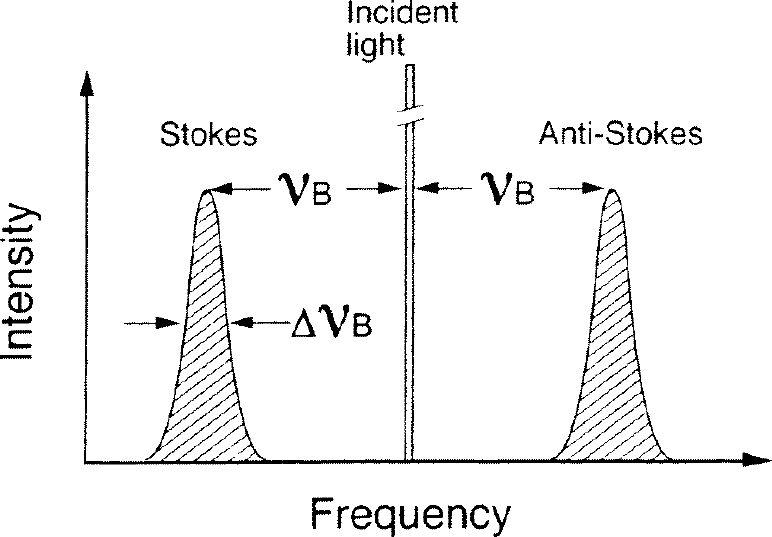
\includegraphics[width=0.6\textwidth]{raman_spectrum.png}
	\caption{Raman scattering spectrum \cite{fer:oks}}
	\label{fig:raman_spectrum}
\end{figure}
Typically, the bandwidth of scattered signals is 20 -- 30 THz. These spectra can be well-approximated by a triangular characteristic. Therefore, $\varDelta E$ should be taken by calculating, or measuring effective wavelengths of Stokes and anti-Stokes spectra. \\

Similar to Brillouin scattering, Raman effect can also be spontaneous or stimulated. In stimulated Raman scattering (abbr. SRS), the pump wave will beat with the spontaneously produced Raman-scattered wave. The beating will induce more molecular oscillations, creating a positive feedback loop to the scattered signal. The phenomenon sets in after the incident optical power crosses the threshold value, defined as
\begin{equation} \label{eq:raman_threshold}
P_\textrm{th} \approx 16 \frac{A_\textrm{eff}}{g_R L_\textrm{eff}} \textrm{.}
\end{equation}
The threshold value for SRS is higher than that of SBS. Occurrence of SRS will degrade temperature measurements. Therefore, in distributed temperature sensing systems based on Raman scattering, one must ensure the optical powers to stay below threshold level.



% --------------------------------------

\setcounter{stranica}{\thepage}
\addtocounter{stranica}{1}

\end{document}